\documentclass{scrreprt}
\usepackage{listings}
\usepackage{underscore}
\usepackage{graphicx}
\usepackage{enumitem}
\usepackage{float}
\usepackage[bookmarks=true]{hyperref}
\usepackage[utf8]{inputenc}
\usepackage[english]{babel}
\graphicspath{{figs/}}
\hypersetup{
    bookmarks=false,
    pdftitle={Software Requirements Specification for ResQ},
    pdfauthor={ResQ Project Team},
    pdfsubject={Software Requirements Specification},
    pdfkeywords={ResQ, crisis coordination, SRS},
    colorlinks=true,
    linkcolor=blue,
    citecolor=black,
    filecolor=black,
    urlcolor=purple,
    linktoc=page
}%
\def\myversion{1.0 }
\date{}
\setlength{\parindent}{0pt}
\setlength{\parskip}{6pt}

% numbered requirement list that keeps counting across groups
\newcounter{fr}
\newcounter{frsave}
\newenvironment{frlist}
  {\begin{list}{\textbf{FR-\arabic{fr}}}{\usecounter{fr}\setcounter{fr}{\value{frsave}}%
   \setlength{\labelwidth}{1.5cm}\setlength{\leftmargin}{1.8cm}%
   \setlength{\itemsep}{3pt}\setlength{\parsep}{2pt}}}
  {\setcounter{frsave}{\value{fr}}\end{list}}

\begin{document}

\begin{flushright}
    \rule{16cm}{5pt}\vskip0.6cm
    \begin{bfseries}
        \Huge{SOFTWARE REQUIREMENTS\\ SPECIFICATION}\\
        \vspace{0.9cm}
        for\\
        \vspace{0.9cm}
        ResQ\\
        \vspace{0.4cm}
        \Large{Crisis Coordination Platform\\ for Emergency Response}\\
        \vspace{0.9cm}
        \LARGE{Version \myversion}\\
        \large
        \vspace{0.9cm}
        Prepared by : Gurnoor Singh Marok (1024170226)\\
        Rishi Gupta (1024170043)\\
        Tamanna Chadha (1027170237)\\
        Kaif Ahmad (1024170255)\\
        \vspace{0.9cm}
        Submitted to : Ms. Anushka\\
        \vspace{0.9cm}
        \\\normalsize {October 15, 2026}
        \vspace{0.6cm}
        \normalsize{Thapar Institute of Engineering and Technology, Patiala}\\
    \end{bfseries}
\end{flushright}

\tableofcontents

% ======================================================================
\chapter{Introduction}

\section{Purpose}
During a local emergency, the hard problem is rarely collecting a report. The hard problem is coordinating many independent actors, each of whom holds only part of the picture. Phone calls, social media messages and spreadsheets leave volunteers, NGOs and suppliers working from different views of the same situation. Two teams may travel to the same address while another request goes unanswered, nobody can tell whether help actually arrived, and the exact address and phone number of a vulnerable person are often circulated far more widely than necessary.

\begin{bfseries}ResQ\end{bfseries} is a web-based crisis coordination platform that addresses these problems. It gives affected people, volunteers, NGOs, resource providers and administrators a single shared, real-time view of who needs help and who is providing it. This document specifies the requirements of version 1.0 of ResQ.

\section{Intended Audience and Reading Suggestions}
This SRS is written for developers, testers, project managers and course evaluators, and also for the NGO coordinators and administrators who would eventually operate the system. The discussion covers the internal, external, functional and non-functional requirements of ResQ.

Readers who want a quick overview should read Chapters 1 and 2. Developers and testers should concentrate on Chapter 3, which lists the functional requirements, and Chapter 4, which lists the quality requirements. Chapter 5 describes maintenance and planned extensions.

\section{Project Scope}
ResQ creates a shared space in which affected people, responders, resource providers and administrators handle each emergency request together.

An \emph{affected person} (or a bystander acting for them) can report an emergency without creating an account. The report contains a category, a description, a location chosen on a map, an optional contact phone number and, optionally, the supplies needed. The system immediately returns a tracking identifier, which the person can use to follow the request, exchange messages with the responder and, finally, confirm that help arrived.

\emph{Administrators} are the central dispatchers. They verify incoming reports, review ranked suggestions of suitable responders, invite a chosen responder, manage emergency categories and incidents, and monitor performance. Administrator accounts are provisioned by the organisation and cannot be created through public registration. Members of NGOs that have themselves been verified may also verify requests, except requests submitted by themselves or by their own organisation.

\emph{Volunteers} and \emph{NGO members} are the responders. They claim verified requests, communicate with the affected person and mark the work as resolved. Members of the same NGO can act on a request claimed by one of their colleagues.

\emph{Resource providers} and \emph{NGOs} hold supplies. They register resources, maintain inventory and allocate supplies against the itemised needs of a request. An allocation is accepted only when the stock actually exists.

\begin{figure}[!htb]
    \centering
    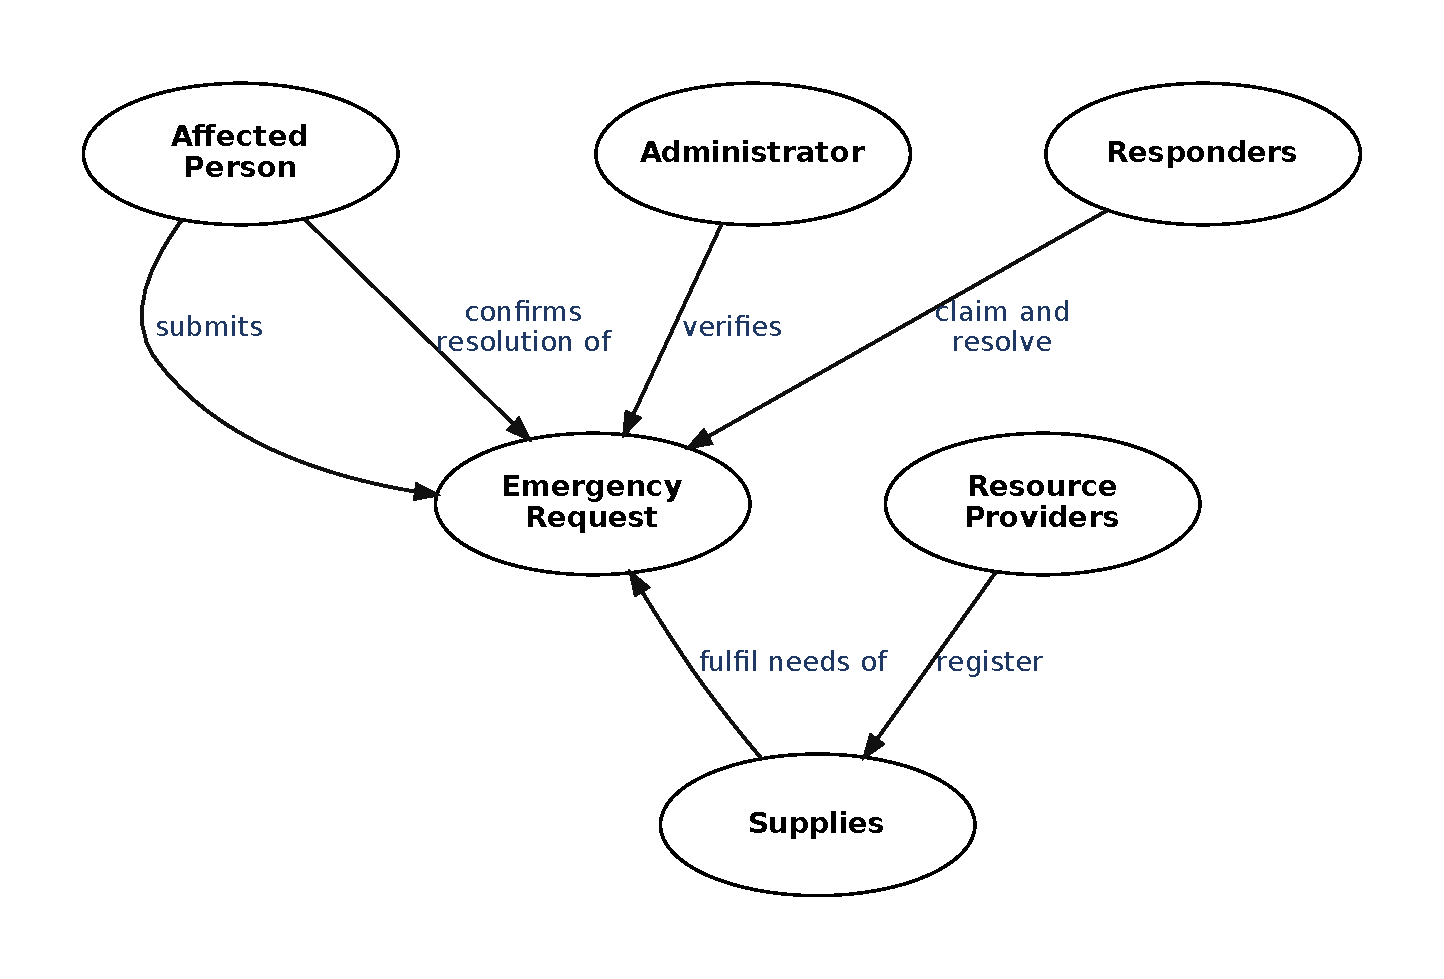
\includegraphics[width=0.52\textwidth]{fig_workflow}
    \caption{Entire work-flow}
    \label{fig:workflow}
\end{figure}

Figure~\ref{fig:workflow} gives an overview of the project and shows how the entities depend on each other.

\emph{Request cycle.} In Figure~\ref{fig:workflow}, the Affected Person submits an Emergency Request; the Administrator verifies it; Responders claim and resolve it; and the Affected Person confirms the resolution, which is what finally closes the request.

\emph{Supply cycle.} Resource Providers register Supplies, and those Supplies are used to fulfil the needs of an Emergency Request.

The system never assigns a responder automatically: matching only suggests and ranks candidates, and a request is claimed only by a responder's own action. Outside the scope of version 1.0 are a native mobile application, SMS or USSD reporting, offline peer-to-peer messaging, online payments and automatic dispatch.

% ======================================================================
\chapter{Overall Description}

\section{Product Perspective}
ResQ replaces the informal channels (phone calls, social media messages, paper lists and spreadsheets) that are normally used to coordinate local emergency response. It is a self-contained web application made of three tiers: a React single-page application in the browser, a stateless Express REST API with a Socket.IO real-time layer, and a MongoDB database that is always the single source of truth. Sockets are used only to push changes to connected screens.

The only external services are the OpenStreetMap tile servers used to draw maps and, optionally, a free-tier language model used to suggest a category for a free-text report. If the language model is disabled or unreachable, a built-in keyword classifier is used and request submission is unaffected. The whole system is built on free or open-source components, so that it can be developed, tested and demonstrated at no cost.

\section{User Classes and Characteristics}
ResQ has five types of users, grouped as follows.
\begin{itemize}
  \item Affected Persons
  \item Responders
    \begin{itemize}
        \item Volunteers
        \item NGO Members
    \end{itemize}
  \item Resource Providers
  \item Administrators
\end{itemize}

\begin{figure}[!htb]
    \centering
    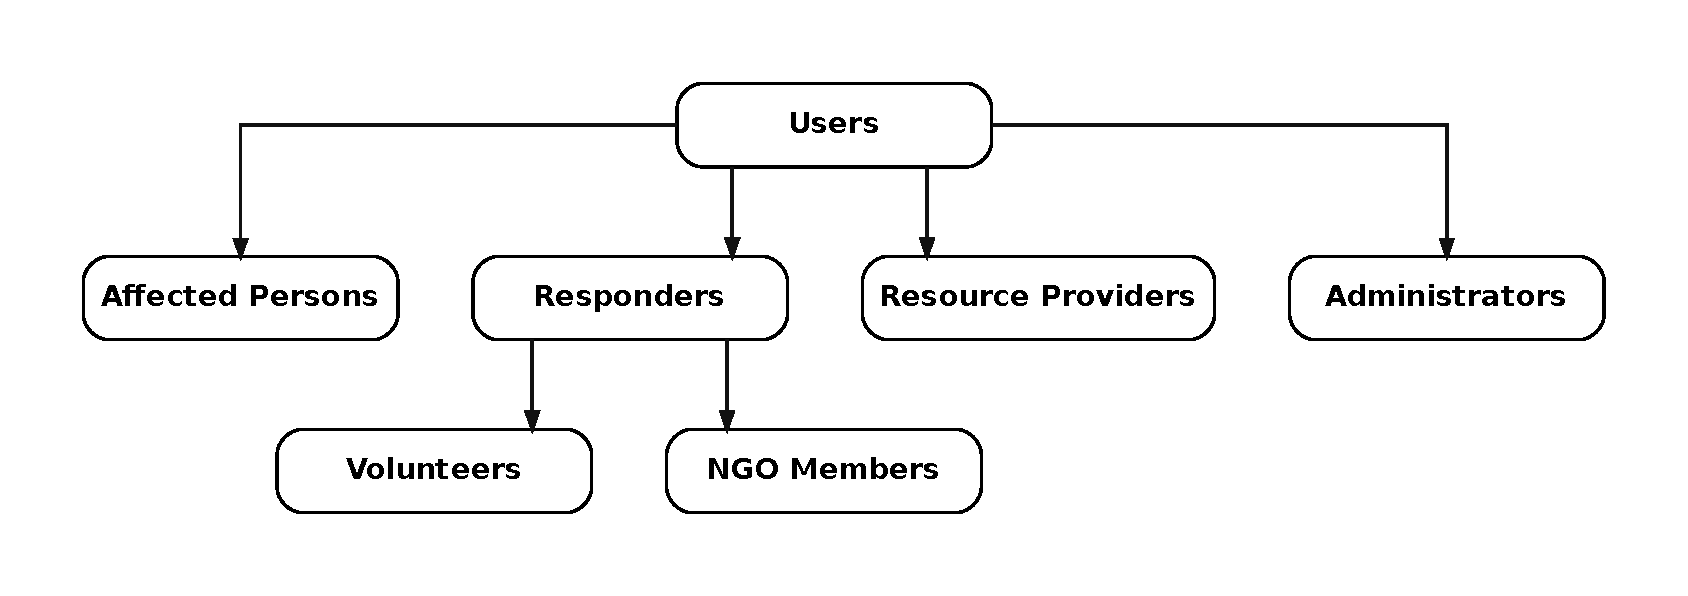
\includegraphics[width=0.7\textwidth]{fig_users}
    \caption{Types of users}
    \label{fig:users}
\end{figure}

\textbf{Affected persons} may be in distress, may have only a mobile phone and a weak connection, and cannot be expected to learn a complex interface. They can use the system without an account. \textbf{Volunteers} are individual field responders, often working from a phone. \textbf{NGO members} work for an organisation with a depot, other members and, optionally, a verified status. \textbf{Resource providers} hold stock such as medical kits, water or blankets, and supply it but do not carry out field rescue. \textbf{Administrators} are trained dispatchers who work from a desktop console.

\section{Product Functions}
ResQ stores every emergency request together with its complete history. Before using any function other than reporting and tracking a request, a user has to register and log in. The main data are described below and shown in Figures~\ref{fig:datacore}, \ref{fig:dataresource} and \ref{fig:datacomm}.

\begin{figure}[!htb]
    \centering
    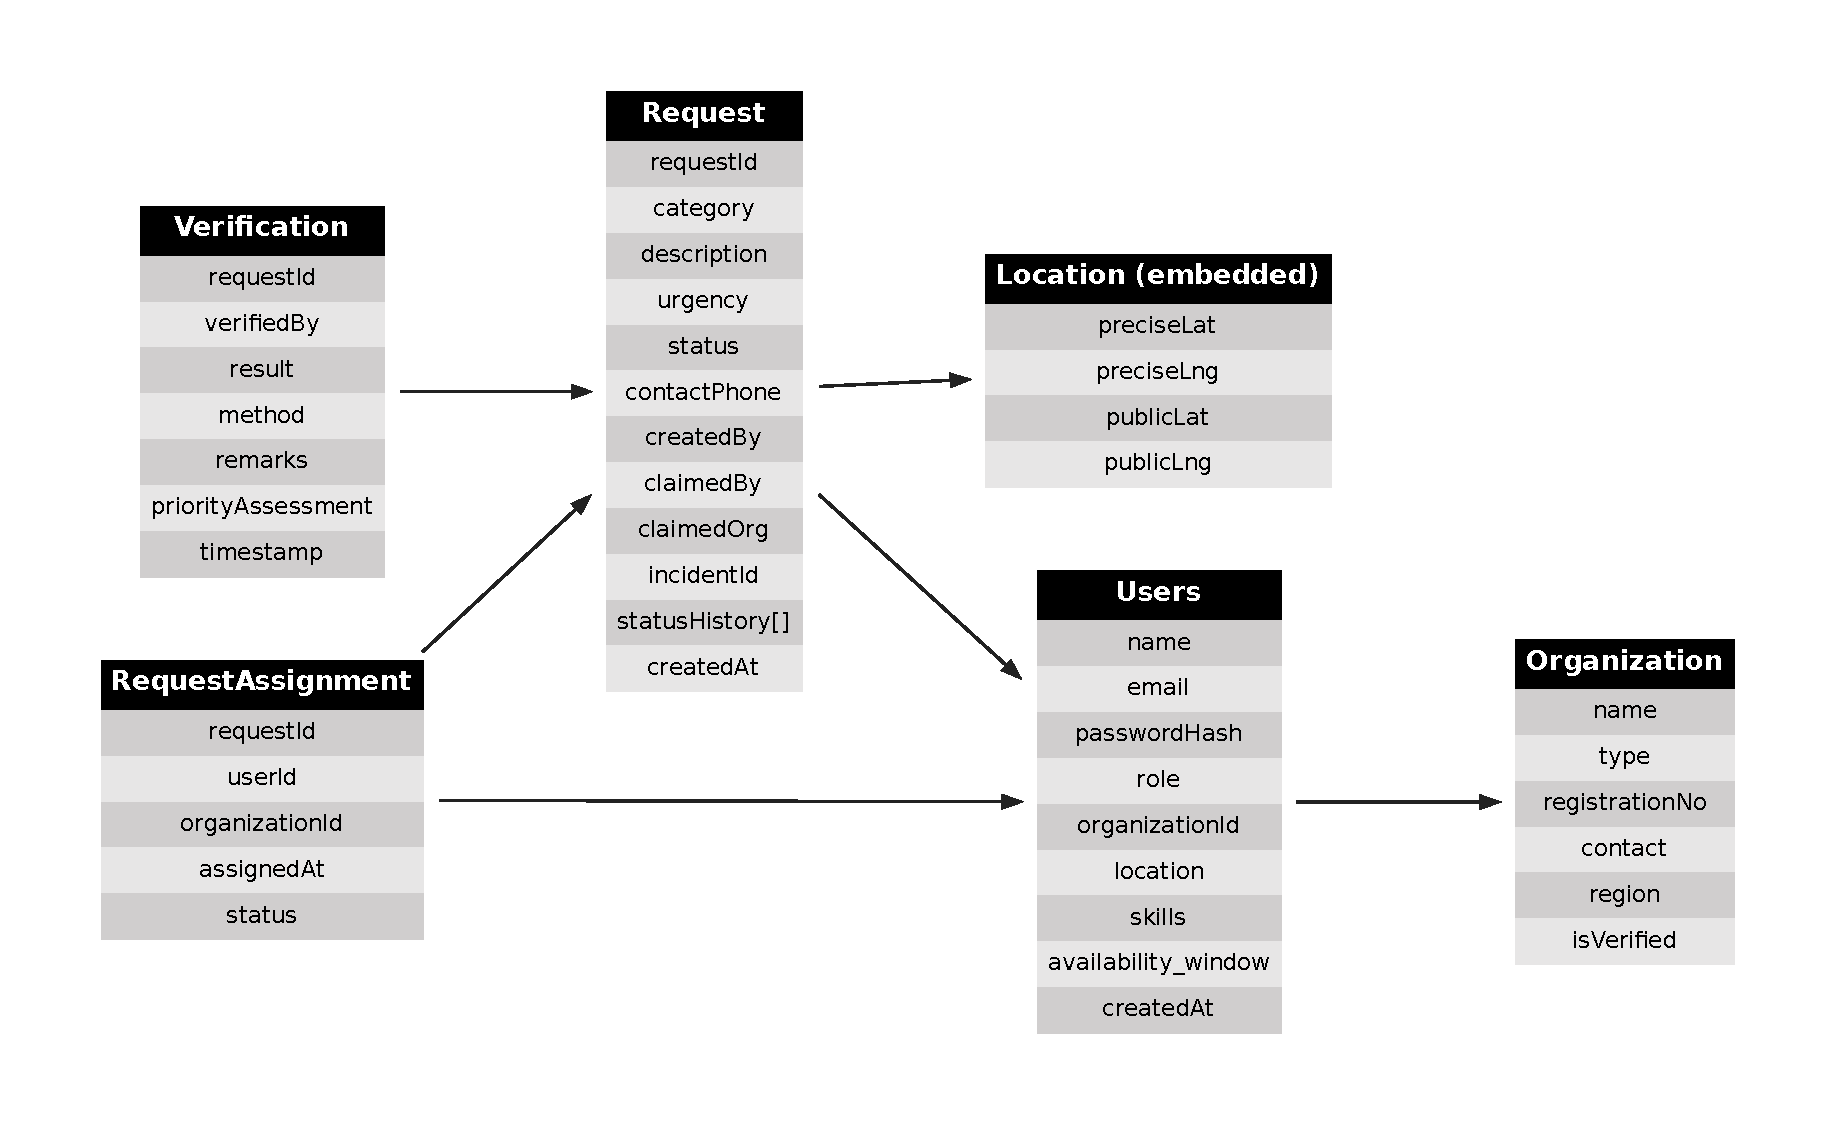
\includegraphics[width=0.88\textwidth]{fig_data_core}
    \caption{Data model: users, requests and verification}
    \label{fig:datacore}
\end{figure}

All users have a name, email, role, password hash (never the password itself), an optional organisation and a creation time stamp. Responders may additionally declare a location, certified skills and a daily availability window, which the matching function uses.

A request has a tracking identifier of the form REQ-YYYY-XXXXXX, a category, a description, an urgency level (low, medium, high or critical), a status, an optional contact phone number, the user who created it, the user and organisation that claimed it, an optional incident and a status history. The status is always one of the following.
\begin{enumerate}
    \item unverified: the report has been received and nobody has checked it yet.
    \item verified: an administrator or a verified NGO has judged the report to be genuine.
    \item in progress: a responder has claimed the request.
    \item resolved: the responder reports that the work is complete.
    \item closed: the affected person has confirmed that help arrived.
    \item cancelled: the request was withdrawn before it was closed.
\end{enumerate}
Each status change appends a history entry containing the new status, the time and the acting user.

The location of a request is stored twice: an exact coordinate pair and a coarse public pair obtained by displacing the exact point by a random offset of up to 0.005 degrees (roughly 500 metres). Only the coarse pair is shown to the general public.

A verification record stores who verified a request, the result (for example verified as legitimate, duplicate, unfounded or needing more information), the method used (phone call, field visit, third-party NGO or cross-reference), free-text remarks and a priority assessment. A request assignment records which responder, and which organisation, took on a request and when.

\begin{figure}[H]
    \centering
    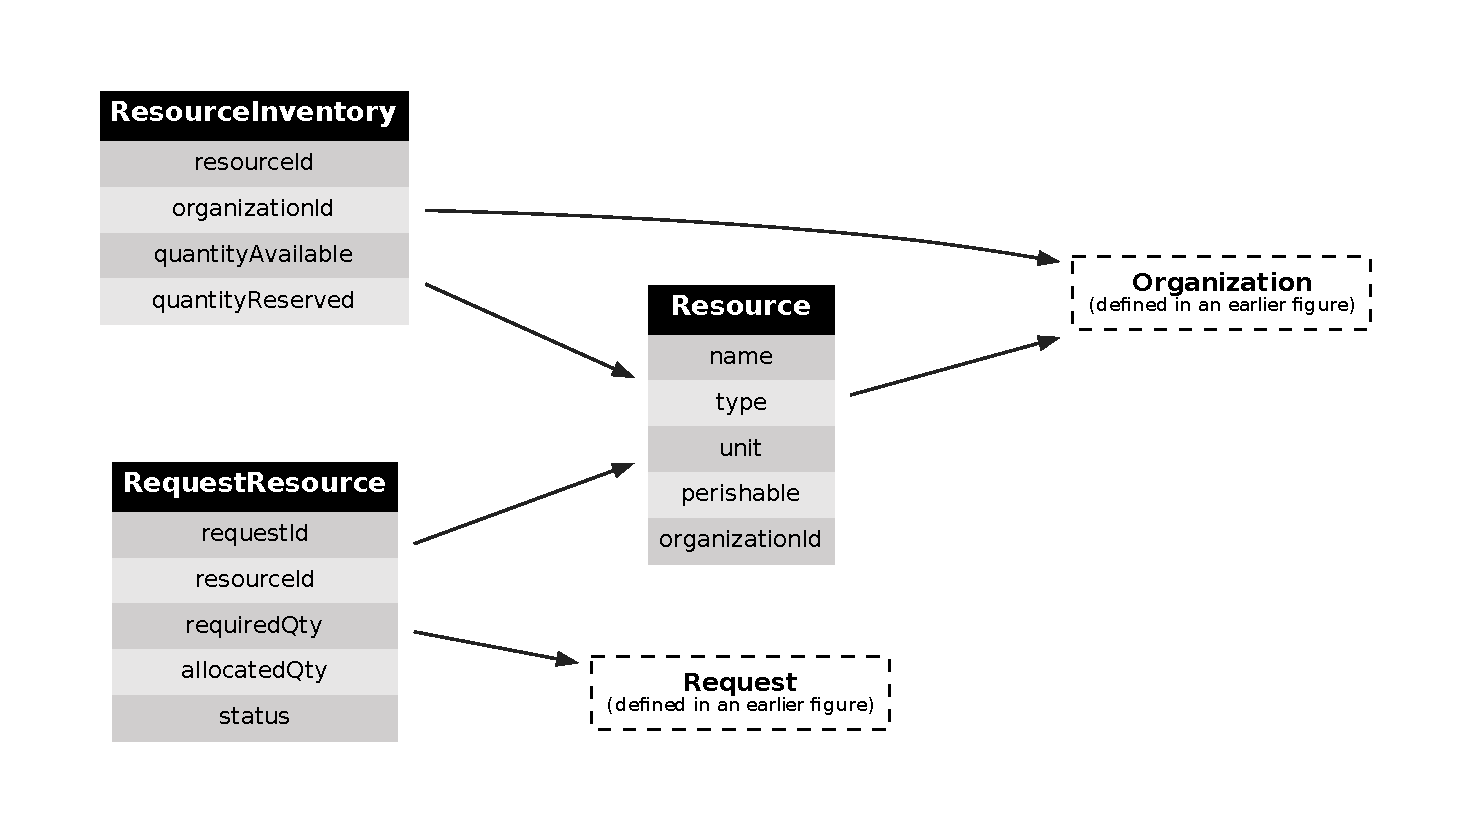
\includegraphics[width=0.68\textwidth]{fig_data_resource}
    \caption{Data model: organisations, resources and inventory}
    \label{fig:dataresource}
\end{figure}

An organisation has a name, type, registration number, contact details, operating region and a verification flag. A resource is a type of supply (for example drinking water or trauma kits) with its unit and perishability. Resource inventory records, for each organisation and resource, the quantity available and the quantity reserved. A request resource records how much of a resource a request requires and how much has been allocated so far.

\begin{figure}[H]
    \centering
    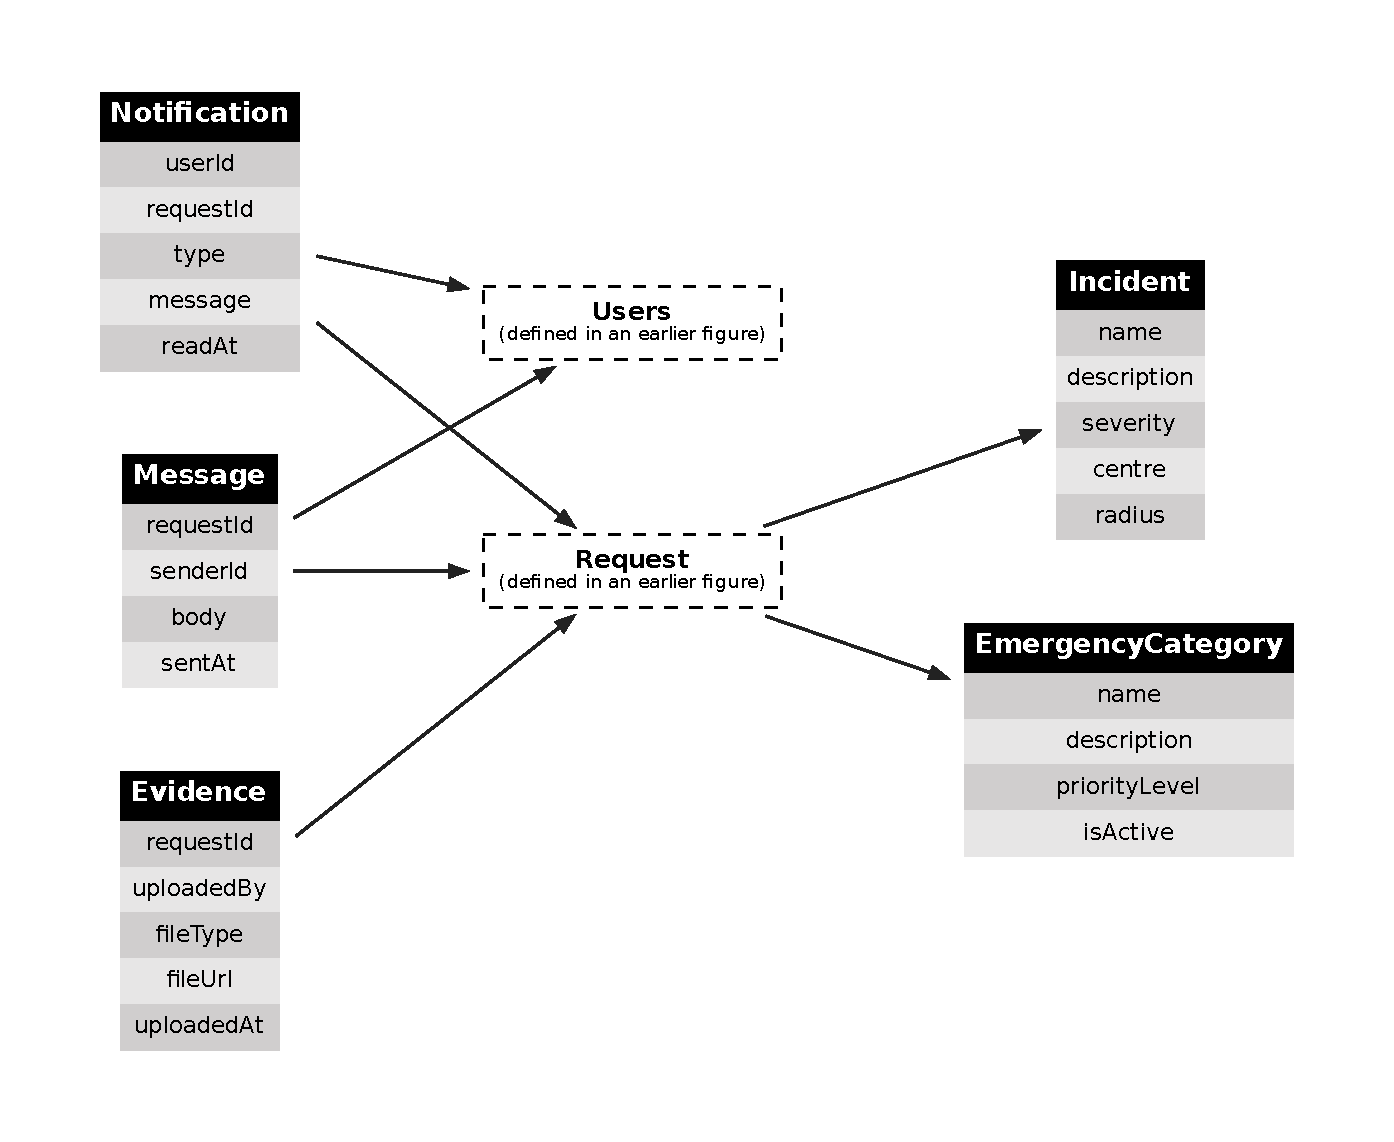
\includegraphics[width=0.55\textwidth]{fig_data_comm}
    \caption{Data model: communication and coordination}
    \label{fig:datacomm}
\end{figure}

Messages belong to a request. Notifications are addressed to a user and may refer to a request. Evidence stores only the metadata of an attached photograph or document, while the file itself is kept in server storage. An incident groups several related requests (for example one flood) and has a name, severity and a circular area. An emergency category has a name, a priority level and an active flag, and is managed by administrators.

\section{Operating Environment}
The website works in any modern web browser (Chrome, Edge, Firefox or Safari) on Windows, macOS, Linux, Android or iOS, and the layout adapts to phone screens. The server requires Node.js and a MongoDB database, and is designed to run on free-tier hosting. An internet connection is needed to load map tiles and to receive live updates.

\section{Design}
The activities of each user class are grouped as follows.

Affected persons have two steps:
\begin{itemize}
    \item Request Submission
    \item Request Tracking
\end{itemize}
The person describes the emergency, marks the place on a map and receives a tracking identifier. On the tracking page they watch the status change live, exchange messages with the responder, may withdraw the request, and finally confirm resolution.

\begin{figure}[H]
    \centering
    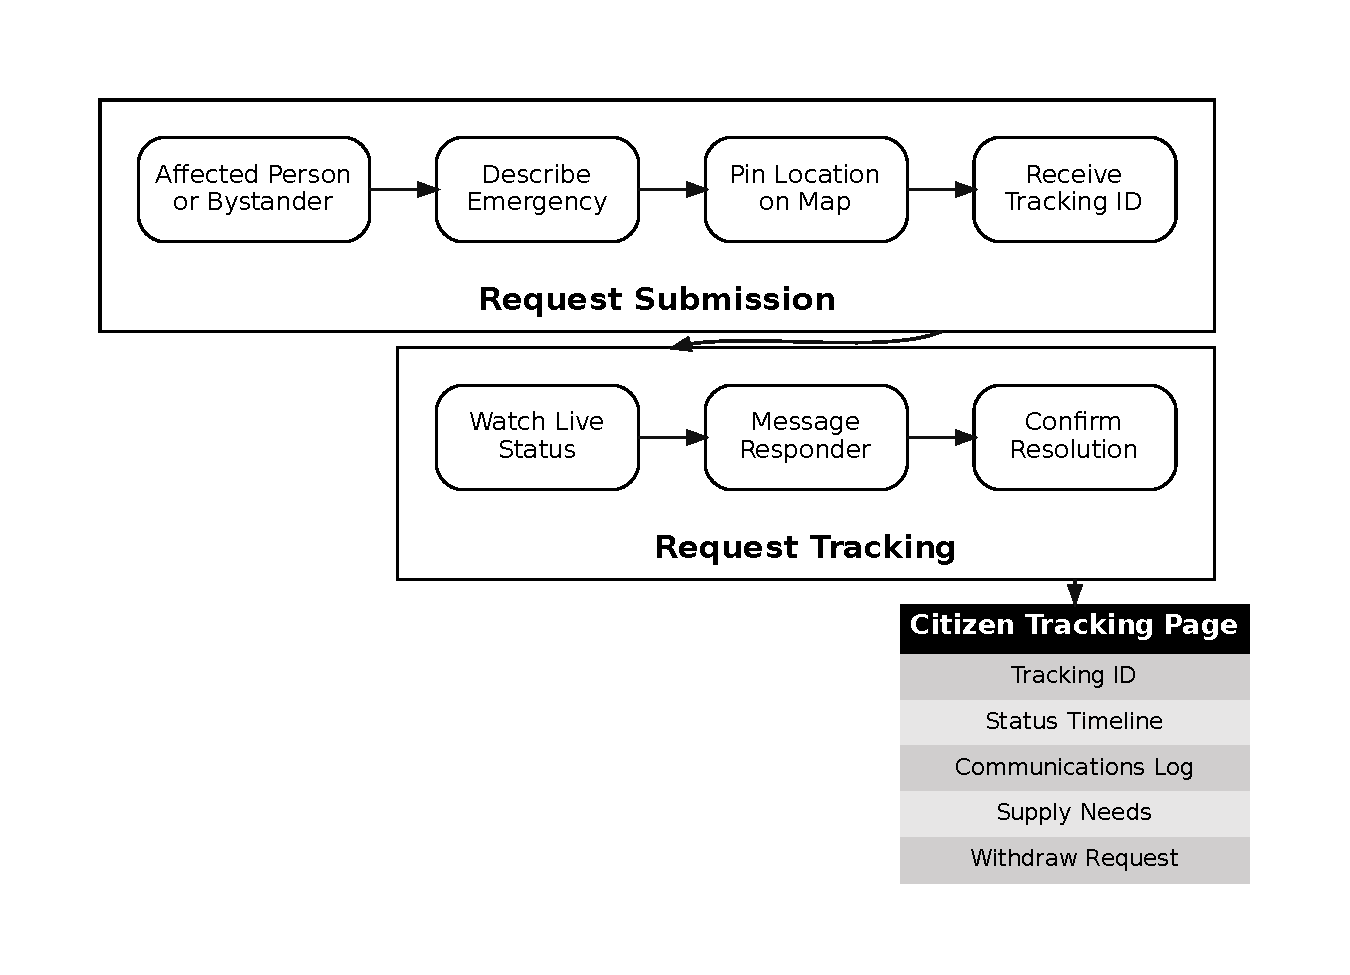
\includegraphics[width=0.6\textwidth]{fig_act_citizen}
    \caption{Citizen activities}
    \label{fig:actcitizen}
\end{figure}

Administrators and responders share one console, a map beside a filterable list of requests, and differ only in the actions available to them. The administrator verifies requests, reviews the ranked suggestions, invites a responder, manages categories and incidents and reads the analytics. The responder claims a request, allocates supplies (NGO members), messages the citizen and marks the work resolved.

\begin{figure}[H]
    \centering
    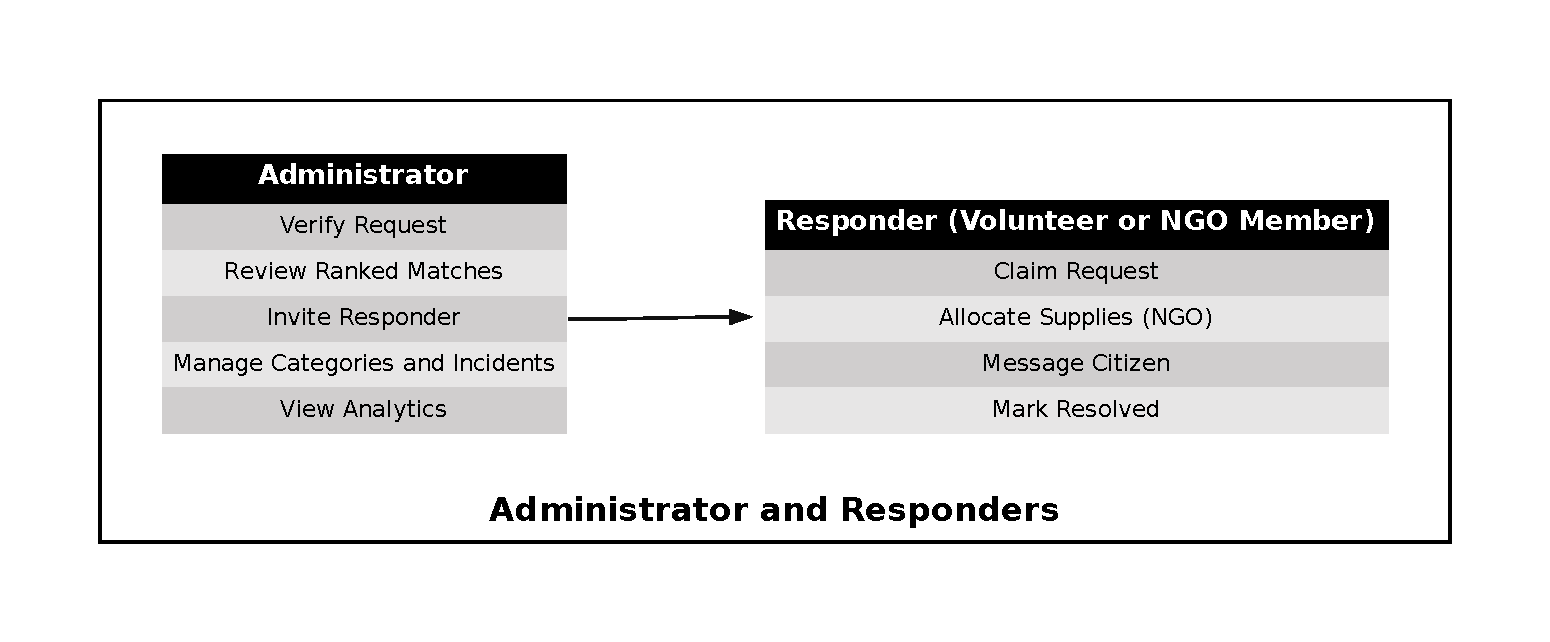
\includegraphics[width=0.75\textwidth]{fig_act_admin}
    \caption{Administrator and responder activities}
    \label{fig:actadmin}
\end{figure}

Resource providers use a depot and inventory dashboard to register resources, manage stock and allocate supplies to requests.

\begin{figure}[H]
    \centering
    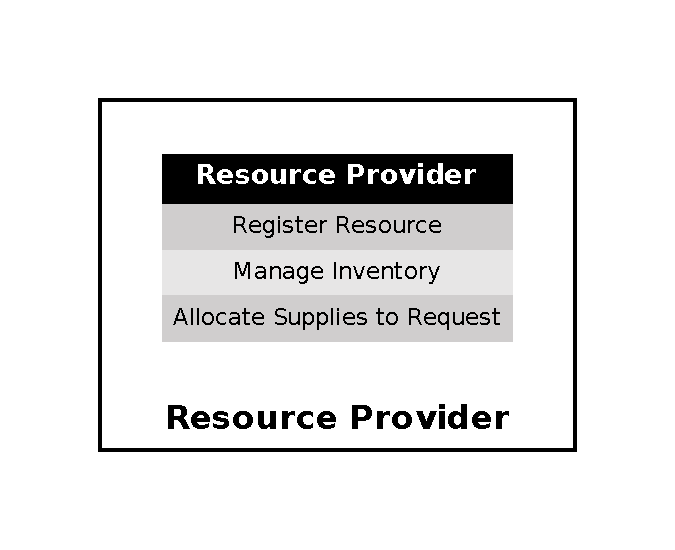
\includegraphics[width=0.3\textwidth]{fig_act_provider}
    \caption{Resource provider activities}
    \label{fig:actprovider}
\end{figure}

The interface follows a calm, high-legibility, dispatch-console style. Colour is used only to show status, and the same colours are used for list markers and map pins. Lists are dense and readable on a phone.

% ======================================================================
\chapter{System Features}
ResQ is a coordination system, so its main purpose is to move each emergency request reliably from report to confirmed resolution while keeping every user's view consistent and protecting the privacy of the people involved.

\section{Description and Priority}
All the features below are part of version 1.0. They are listed from the highest to the lowest priority.
\begin{enumerate}
    \item Emergency Request Submission and Tracking: the goal feature of the system. Anyone can report an emergency and follow it, without an account.
    \item Verification and Lifecycle Control: every request passes through the enforced sequence of statuses, and only authorised users can move it forward.
    \item Claiming, Resolution and Confirmation: responders claim and resolve requests, and only the affected person can close them.
    \item Privacy-Preserving Location Handling: exact location and phone number are revealed only to authorised users.
    \item Real-Time Updates: every connected screen shows status changes without a manual refresh.
    \item Resource Inventory and Allocation: supplies are registered, tracked and allocated against real stock.
    \item Communication: request-scoped messaging, in-app notifications and evidence attachments.
    \item Matching Suggestions: ranked, explainable suggestions of suitable responders. The system suggests and never assigns.
    \item Incident, Category and Organisation Management.
    \item Analytics: the measures used to evaluate the system.
    \item Free-Text Classification: an optional hint that never blocks submission.
\end{enumerate}

\section{Functional Requirements}
The requirements below use the word \emph{shall} for mandatory behaviour.

\subsection*{Accounts and access}
\begin{frlist}
    \item The system shall allow anyone to submit and track an emergency request without an account.
    \item The system shall allow affected persons, volunteers, NGO members and resource providers to register themselves. It shall not allow administrator accounts to be created through public registration.
    \item The system shall authenticate registered users by email and password, store only a salted bcrypt hash of the password, and issue a signed JSON Web Token on login.
    \item The system shall check the role of the caller on the server for every protected action, in addition to any restriction in the interface.
\end{frlist}

\subsection*{Request submission}
\begin{frlist}
    \item The system shall accept a category, a description, a location chosen on a map, an optional contact phone number and optional itemised supply needs.
    \item The system shall generate a unique tracking identifier of the form REQ-YYYY-XXXXXX and return it immediately.
    \item The system shall offer only the categories that administrators have marked active.
    \item The system shall, where the optional classifier is available, suggest a category and an urgency level from the description. The suggestion shall be dismissible, shall never override the person's own choice, and shall never delay or block submission.
\end{frlist}

\subsection*{Lifecycle}
\begin{frlist}
    \item The system shall keep each request in exactly one of the statuses unverified, verified, in progress, resolved, closed or cancelled, and shall reject any attempt to skip or reverse a stage.
    \item The system shall allow a request to be verified by an administrator or by a member of an organisation whose verification flag is set, recording the result, method, remarks and priority assessment.
    \item The system shall refuse verification by the user who submitted the request, and by any member of the submitter's organisation.
    \item The system shall allow only volunteers and NGO members to claim a request, only when it is verified, and only through an explicit action.
    \item The system shall allow a request to be marked resolved by its claimant, by an administrator, or by a member of the claiming organisation.
    \item The system shall allow a request to be closed only by the affected person's confirmation, using their account or the phone number given at submission. Neither an administrator nor a responder shall be able to close it.
    \item The system shall allow the requester to withdraw a request that is not yet resolved or closed, and an administrator to withdraw a request before it is closed.
    \item The system shall append an entry to the status history of the request at every status change.
\end{frlist}

\subsection*{Privacy}
\begin{frlist}
    \item The system shall store both the exact location and a coarse public location displaced by a random offset of up to 0.005 degrees.
    \item The system shall return the exact coordinates and the contact phone number only to an administrator, to the original requester and to the assigned claimant. All other callers shall receive only the coarse location.
    \item The system shall apply the same redaction to data pushed over real-time connections.
\end{frlist}

\subsection*{Real-time behaviour}
\begin{frlist}
    \item The system shall push new requests, status changes, allocation changes, messages and notifications to the relevant connected users without a manual refresh, and only after the database write has succeeded.
    \item The system shall let a client that reconnects after a network interruption resynchronise its data from the REST interface, so that the database remains the single source of truth.
\end{frlist}

\subsection*{Resources and inventory}
\begin{frlist}
    \item The system shall allow resource providers and NGOs to register resources and maintain available and reserved quantities, only for an organisation to which they belong.
    \item The system shall allow supply needs to be added to a request only by its requester, by an administrator or by its claimant.
    \item The system shall allow only NGOs and resource providers to allocate supplies to a request, shall reject an allocation that exceeds the unreserved stock, and shall update the stock in the same operation.
    \item The system shall allow only resource providers, NGOs and administrators to reserve or release inventory.
    \item The system shall show, for each required item, how much has been allocated against how much is needed.
\end{frlist}

\subsection*{Communication}
\begin{frlist}
    \item The system shall provide a message thread for each request. Before the request is claimed, only the administrator and the requester may use it. After it is claimed, the claimant, the requester, the administrator and members of the claiming organisation may use it.
    \item The system shall let a requester without an account unlock the thread by entering the phone number used at submission.
    \item The system shall create in-app notifications, with a read and unread state, for verification, claiming, resolution, new messages and invitations.
    \item The system shall allow evidence (photographs or documents) to be attached to a request, storing the file type, the uploader and the time.
\end{frlist}

\subsection*{Coordination and administration}
\begin{frlist}
    \item The system shall rank candidate responders and providers for a verified request using a weighted score of proximity (35\%), suitability (30\%), capacity (20\%) and availability (15\%), treating undeclared availability or location as neutral, and shall show the contribution of each factor.
    \item The system shall allow administrators and NGO coordinators to invite a suggested candidate by notification. An invitation shall not claim the request on the candidate's behalf, and a duplicate invitation shall be rejected.
    \item The system shall allow administrators to create incidents with a name, severity, description and radius, to link requests to them and to list the requests of an incident.
    \item The system shall allow administrators to create emergency categories, set their priority and activate or deactivate them.
    \item The system shall provide an organisation directory that can be filtered by region and type, and shall let NGOs and response units register their organisation profile.
\end{frlist}

\subsection*{Analytics and interface}
\begin{frlist}
    \item The system shall provide administrators with a dashboard that reports Time-to-Match, double-booking rate, confirmation rate and real-time propagation latency over the last 24 hours, 7 days, 30 days or all time.
    \item The system shall provide one console, a map beside a filterable list of requests, for all signed-in roles, with map markers coloured by status. At phone widths the map and the list shall be presented as tabs.
    \item The system shall provide a public home page that explains the purpose and workflow of ResQ.
\end{frlist}

\subsection*{Technology}
ResQ is built with the following technologies.
\begin{itemize}
    \item Front-End: React 18, TypeScript, Vite, Tailwind CSS, react-leaflet with OpenStreetMap tiles.
    \item Back-End: Node.js, Express, TypeScript, Socket.IO, JSON Web Tokens and bcrypt.
    \item Database: MongoDB (Atlas free tier) with Mongoose.
    \item Testing: Vitest and Supertest for the server, Playwright for end-to-end tests.
    \item Optional classification: Google Gemini (free tier) with a built-in keyword classifier as fallback.
\end{itemize}

% ======================================================================
\chapter{Other Nonfunctional Requirements}

\section{Performance Requirements}
Because ResQ is used in emergencies, delay in the system directly delays help. The performance targets are the following.
\begin{itemize}
    \item Time-to-Match, the time from a request being verified to it being claimed, shall have a median of at most 15 minutes during pilot testing.
    \item Real-time propagation latency, the time from a change being saved to it appearing on the other connected screens, shall be under 2 seconds, with no missed updates.
    \item The double-booking rate, the share of resources assigned to more than one active request at the same time, shall be 0\%.
    \item Submission, claiming and status updates shall be available at least 99\% of the time during pilot hours.
    \item The confirmation rate, the share of resolved requests that reach the closed status through the requester's confirmation, shall be measured and reported.
\end{itemize}
The system keeps the API stateless and keeps the database as the single source of truth, so that the real-time layer can be scaled without risking inconsistent data. In a single-operator pilot run on one machine, the measured median propagation latency was 23 ms (95th percentile 29 ms) and no double booking occurred.

\section{Security Requirements}
\begin{itemize}
    \item Apart from submitting and tracking a request, only registered and authenticated users can use the system. A user can perform only the actions allowed for their role, and this is enforced on the server.
    \item Passwords are stored only as bcrypt hashes. Tokens are signed with a secret that is read from the environment and is never kept in the source code.
    \item The exact location and phone number of an affected person are hidden from everyone except the administrator, the requester and the assigned claimant, in both the REST interface and the real-time channel.
    \item A user shall not verify a request that they or their own organisation submitted.
    \item Administrator accounts cannot be created by self-registration.
    \item Real-time connections are authenticated with the same token as the REST interface, and a user receives messages only for the requests that user is authorised to see.
    \item Cross-origin access is limited to the application's own front end, and the hosting platform encrypts traffic in transit.
\end{itemize}

\section{Software Quality Attributes}
\begin{itemize}
    \item \textbf{Reliability:} every change is written to the database before it is broadcast, and the REST interface continues to work if the real-time layer fails.
    \item \textbf{Graceful degradation:} the optional classifier can be disabled or can fail without any effect on submission.
    \item \textbf{Usability:} plain, active-voice wording, dense and readable lists, and a layout that works on a phone.
    \item \textbf{Maintainability:} strictly typed TypeScript code, separate front end and back end, and one central code path for status changes.
    \item \textbf{Testability:} at the time of writing, 115 automated server tests in 20 test files and 5 Playwright end-to-end scenarios cover the lifecycle, the role permissions, the matching, the analytics and the real-time behaviour.
    \item \textbf{Portability:} the front end runs in any modern browser, and the server runs wherever Node.js and MongoDB are available.
    \item \textbf{Cost:} no paid service is required to build, test, run or demonstrate the system.
\end{itemize}
Database, logical and user-interface testing are all required.

\section{Business Rules}
\begin{itemize}
    \item A request can be claimed only after it has been verified.
    \item A request can be closed only when the affected person confirms that help arrived.
    \item The system suggests but never assigns. A responder is committed only through that responder's own action.
    \item Supplies can be allocated only from stock that actually exists.
    \item Precise location and contact details are revealed only to authorised users.
    \item Every status change is recorded and cannot be removed.
\end{itemize}

% ======================================================================
\chapter{Other Requirements}
ResQ needs maintenance as the way emergencies are managed changes over time. The code base is kept modular so that features can be added without disturbing the lifecycle rules.

The following extensions are planned for later versions.
\begin{itemize}
    \item An offline submission queue, so that a report written without network coverage is saved on the device and sent automatically when a connection returns.
    \item SMS or USSD reporting for people with basic phones, which needs a gateway that is not free and is therefore outside version 1.0.
    \item Direct assignment by a dispatcher with an accept and decline step, so that no responder is ever committed silently.
    \item A simplified landing page for affected persons that shows only their own requests.
    \item Normalisation of phone numbers, so that different formats of the same number are accepted.
    \item A pilot with independent participants, larger than the single-operator pilot completed so far.
\end{itemize}
The system shall collect only the personal data that is needed to coordinate a response. Deployment on free-tier hosting may cause a slow first response after a period of inactivity, and this is accepted for the educational setting.

\end{document}
